\chapter{Results}
Discussion of the results takes place in this chapter. The chapter begins with
with a description of the data collection process, followed by the parameters
considered for performance analysis and ends with discussion of the results obtained.

\section{Data Collection}
With \textit{CreateDatafile} function of each device class, which is called in the
\textit{Install} function of the helper classes, log files are created to contain
data loss and packet delay values of each device simulated. Packet delay and data
loss are the parameters of interest to evaluate the performance of APT-MAC.
\begin{enumerate}
    \renewcommand{\labelenumi}{}
\item \textit{Packet Delay:} the difference in time between generating a packet data
    and sending to the reader.\\
    A call to \textit{SetPacketGeneratingTime} function at the end of
    \textit{GeneratePacket} function sets the time of packet generation and when a
    packet is sent to the reader, \textit{SetPacketSentTime} is called to set the
    sending time. The difference is thus the packet delay which is log in the packet
    delay log file.
\item \textit{Data Loss:} this is the produced data that is not delivered to the
    reader. Calculated by dividing the amount of data sent by the quantum of data
    produced, the percentage of the result subtracted from $1$ is the data loss.
    Thus it is a percentage.\\
    A counter, \textit{m\_newDataCountProduced}, is kept which is increased,
    a call to \textit{UpdateNewDataProduced()}, anytime a new data is
    produced. The variable, \textit{m\_newDataCountSent}, is increased by a call to
    \textit{UpdateNewDataSent}(), whenever a data packet is sent across to
    the reader. When \textit{m\_queryCounter}, holds the number of
    times a query is received from the reader by a device and increased with a call
    to \textit{UpdateQueryCounter()}, gets to $5$, \textit{data loss} is computed
    as indicated earlier and the value log in the data loss log file. The data loss
    is calculated after every $5$ \textit{data-query} request received by the
    tag-augmented sensor device.
\end{enumerate}
\begin{table}[h!]
    \caption{WORKLOAD SCENARIOS DESCRIPTION}
    \label{tab:WSD}
    \centering
    \begin{tabular} { | c | c | c | c | c | }
        \hline
        \multicolumn{1}{| c }{No. of Sensors}  & \multicolumn{1}{c }{Scenario}
                                             & \multicolumn{1}{ c }{Joystick}
                                             & \multicolumn{1}{ c }{Remote}
                                             & \multicolumn{1}{ c |}{Env. Sensors} \\
        \hline
        \hline
        \multirow{4}{*}{20} & Case 1 & 1 & 2 & 17 \\ 
                            & Case 2 & 2 & 3 & 15 \\ 
                            & Case 3 & 3 & 3 & 14 \\ 
                            & Case 4 & 4 & 4 & 12 \\
        \hline
        \multirow{4}{*}{30} & Case 1 & 1 & 2 & 27 \\
                            & Case 2 & 2 & 3 & 25 \\
                            & Case 3 & 3 & 3 & 24 \\
                            & Case 4 & 4 & 4 & 22 \\
        \hline
        \multirow{4}{*}{40} & Case 1 & 1 & 2 & 37 \\
                            & Case 2 & 2 & 3 & 35 \\
                            & Case 3 & 3 & 3 & 34 \\
                            & Case 4 & 4 & 4 & 32 \\
        \hline
    \end{tabular}
\end{table}
The number of packet producing devices (tag-augmented sensor devices) used for the
gathering of data and to evaluate the performance of APT-MAC was based on table
\ref{tab:WSD}. Environment Sensors included the presence and temperature sensors.
\section{Discussion of Results}
Figure \ref{fig:transcient} depicts the transient time, - duration for APT-MAC device
to get into optimum performance of reduced data loss and packet delay. The transient
time connotes the speed of APT-MAC.\\\\
It takes approximately $50$\textit{ms} to get the data loss of a joystick to less
than $15\%$, the designated optimum threshold. That of a presence sensor, on average,
it takes $0.283$\textit{s} and with the temperature sensor, it quickly reduces the
loss rate at approximately a milli of a second. The data loss of the remote does not
get pass the threshold. 
\begin{center}
    \begin{figure}[h!]
        \centering
        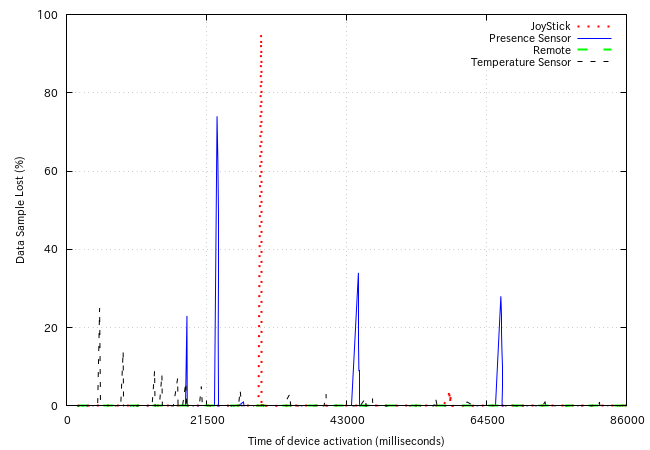
\includegraphics[width=1\linewidth]{transcient}
        \caption{Transient Time of Devices.}
        \label{fig:transcient}
    \end{figure}
\end{center}
The start times are that of the beginning of data production, which indicates the
powering on of the sensory devices.\\\\
APT-MAC gets better when it is run for a longer time. When the running time for an
APT-MAC device is maximized, the better the protocol gets. It can been seen from
figures \ref{fig:20-D-DLSR} and \ref{fig:20-D-DL}, TDMA protocol performs better in
the cases 3 and 4 of the short run for 20 devices \ref{tab:WSD}.\\\\
\newline
\begin{center}
    \begin{figure}[p]
        \begin{subfigure}{1\textwidth}
            \centering
            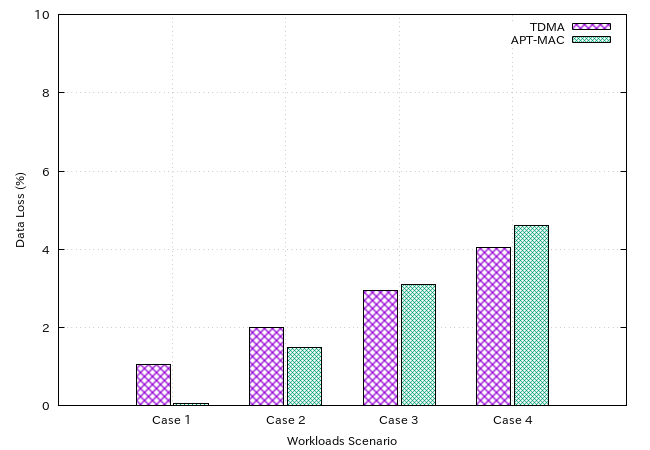
\includegraphics[width=0.8\linewidth]{20-1-data-loss-short-period}
            \caption{20 Devices : Data Loss Short Run.}
            \label{fig:20-D-DLSR}
        \end{subfigure}
        \begin{subfigure}{1\textwidth}
            \centering
            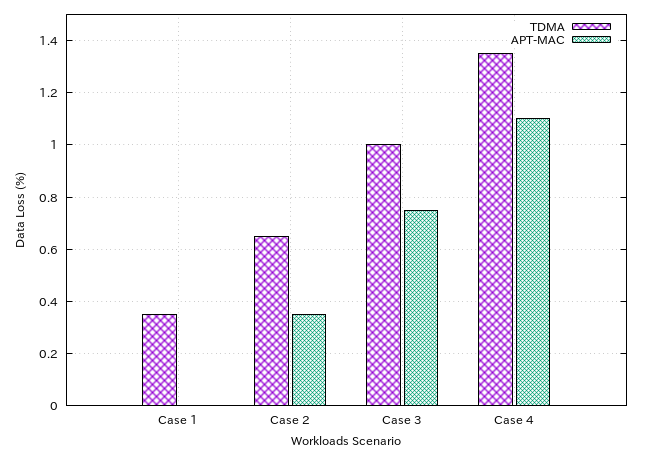
\includegraphics[width=0.8\linewidth]{20-1-data-loss}
            \caption{20 Devices : Data Loss}
            \label{fig:20-D-DL}
        \end{subfigure}
        \begin{subfigure}{1\textwidth}
            \centering
            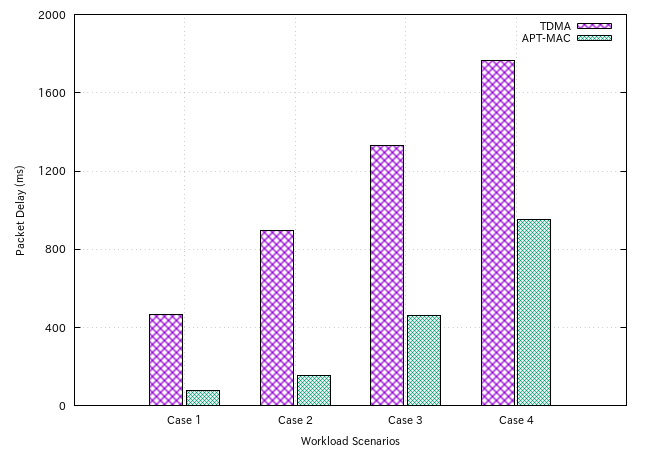
\includegraphics[width=0.8\linewidth]{20-1-packet-delay}
            \caption{20 Devices : Packet Delay}
            \label{fig:20-D-PD}
        \end{subfigure}
    \end{figure}
    \begin{figure}[p]
        \begin{subfigure}{1\textwidth}
            \centering
            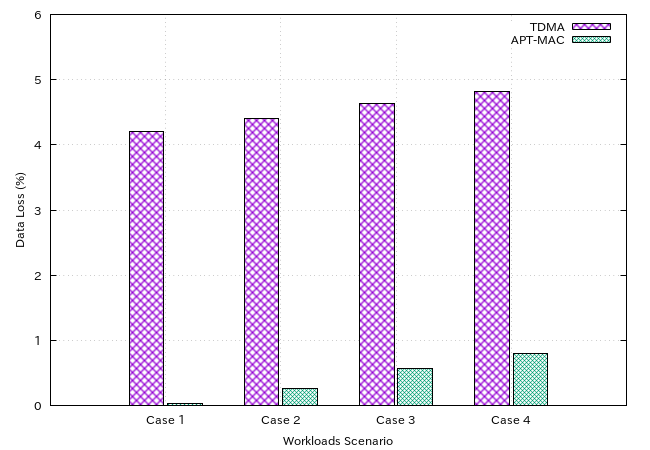
\includegraphics[width=1\linewidth]{30-data-loss}
            \caption{30 Devices : Data Loss}
            \label{fig:30-D-DL}
        \end{subfigure}
        \begin{subfigure}{1\textwidth}
            \centering
            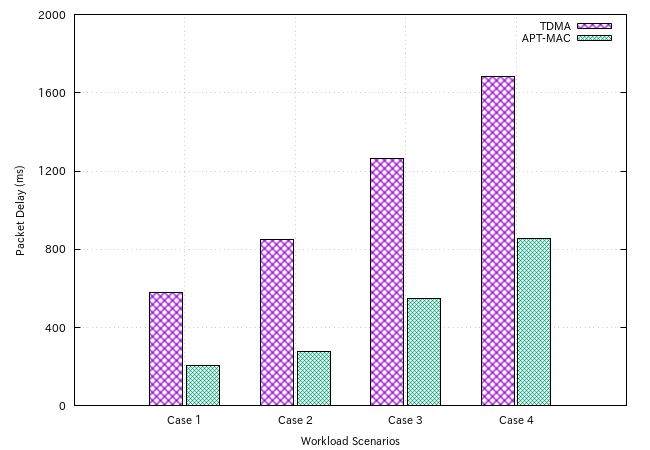
\includegraphics[width=1\linewidth]{30-packet-delay}
            \caption{30 Devices : Packet Delay}
            \label{fig:30-D-PD}
        \end{subfigure}
    \end{figure}
    \begin{figure}[p]
        \begin{subfigure}{1\textwidth}
            \centering
            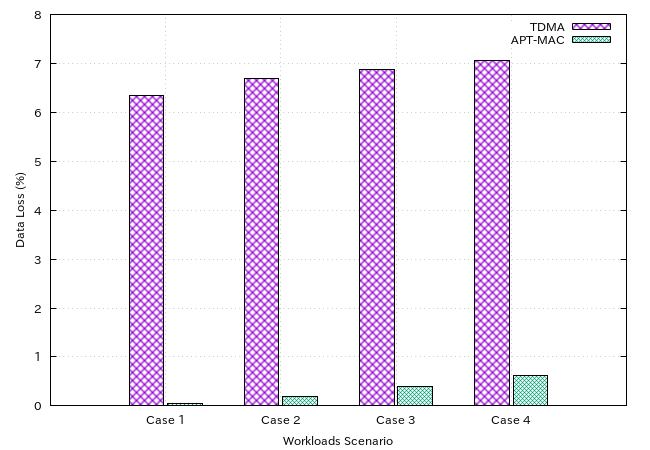
\includegraphics[width=1\linewidth]{40-data-loss}
            \caption{40 Devices : Data Loss}
            \label{fig:40-D-DL}
        \end{subfigure}
        \begin{subfigure}{1\textwidth}
            \centering
            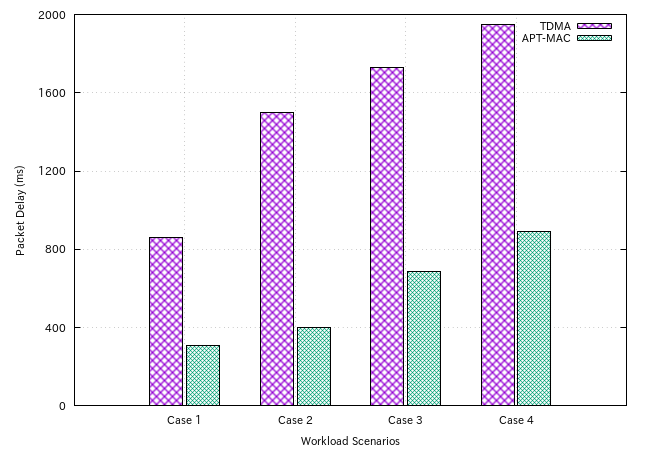
\includegraphics[width=1\linewidth]{40-packet-delay}
            \caption{40 Devices : Packet Delay}
            \label{fig:40-D-PD}
        \end{subfigure}
    \end{figure}
\end{center}
Packet delay, urgency to which packets are delivered to the reader in an equilibrium
state, for 20 devices of the various cases in table \ref{tab:WSD} is shown in figure
\ref{fig:20-D-PD}.
In both APT-MAC and TDMA, the time it takes to deliver new data
almost doubles from case 1 to case 2. It doubles for APT-MAC and almost plateaus for
TDMA in cases 3 to 4. Generally, APT-MAC delivers new data faster with a worse case
(case 4) time of $0.9$\textit{s} while that of TDMA is $1.7628$\textit{s}. On the
average, APT-MAC delivers new packet $2.7$ faster compared to TDMA - average of
$1.115$\textit{s} for TDMA and $0.411$\textit{s} for APT-MAC. Figure
\ref{fig:30-D-PD} and \ref{fig:40-D-PD} show packet delay for 30 and 40 devices 
respectively, similar trend is seen as that of 20 sensory devices with a gradual
increases as number of sensory devices increases.\\\\
Figure \ref{fig:20-D-DL} depicts the data loss, percentage of new data that is lost
as a result of untimely query, for 20 devices.
TDMA losses between $0.35\%$ in case 1 to $1.35\%$ in case 4 while APT-MAC does not
lose any new data in case 1 and the worse case, case 4, losses $1.10\%$. The data
loss doubles across the various cases for both protocols. The trend is similar as the
number devices increases - 30 \& 40 devices - figures \ref{fig:30-D-PD} and
\ref{fig:40-D-PD}, with the data loss of the APT-MAC being $0.8\%$ and $0.625\%$ for
30 \& 40 devices respectively. Proving that the more the sensory devices are the
better APT-MAC gets which is contrary to TDMA.


























